% Preamble
% ---
\documentclass{article}

% Packages

\usepackage{graphicx}
\usepackage{subfig}
\usepackage{pgfplots}

\usepackage{multicol}
\usepackage{float}

\usepackage{tikz}
\usetikzlibrary{shapes.geometric, arrows}

\usepackage[english]{babel}

\usepackage{geometry}
\geometry{margin=1.2cm}

% ---


\graphicspath{ {assets/} }

\setlength{\columnsep}{0cm}
\begin{document}


\section{Face detection}

\begin{multicols}{2}[columnsep=2cm]

% -- Part 1 - Image section
\begin{multicols}{2}
  \centerline{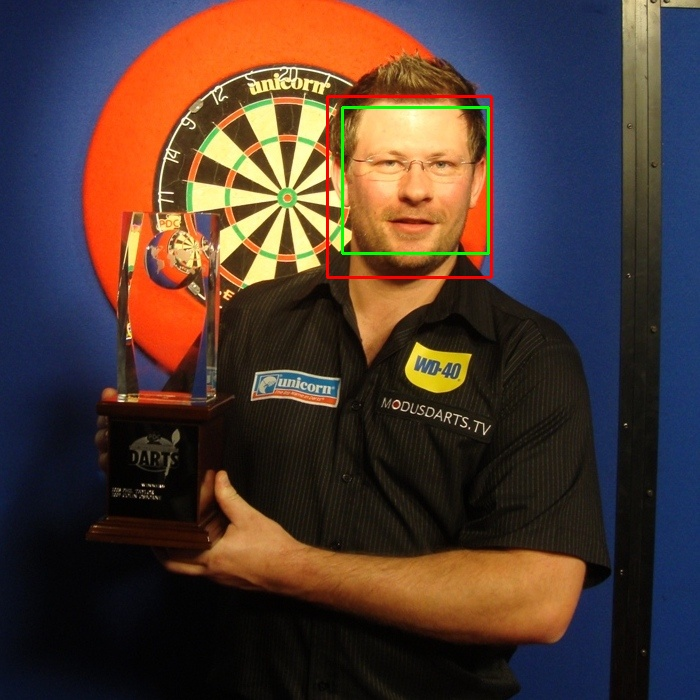
\includegraphics[width=\linewidth]{dart4-face.jpg}\par}
  \centerline{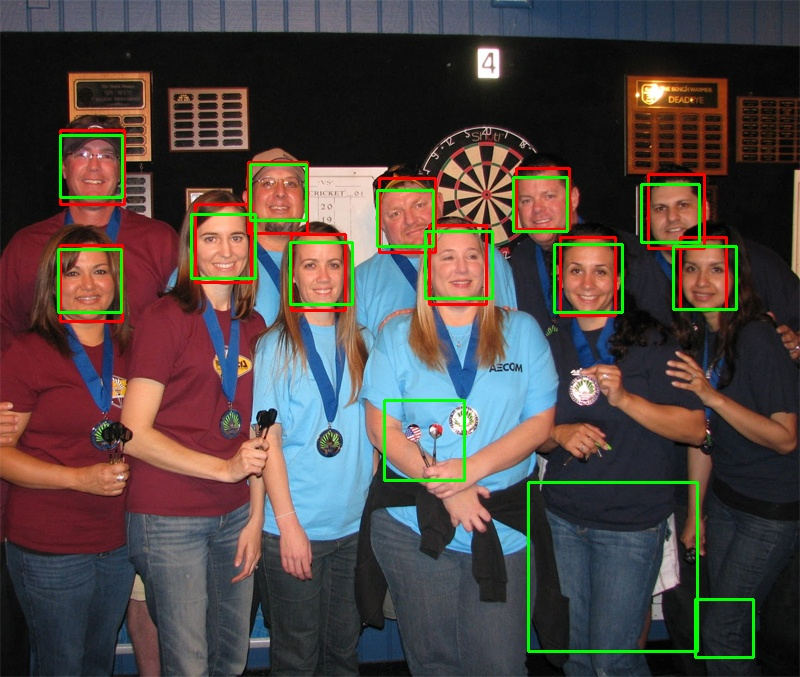
\includegraphics[width=\linewidth]{dart5-face.jpg}\par}
  \centerline{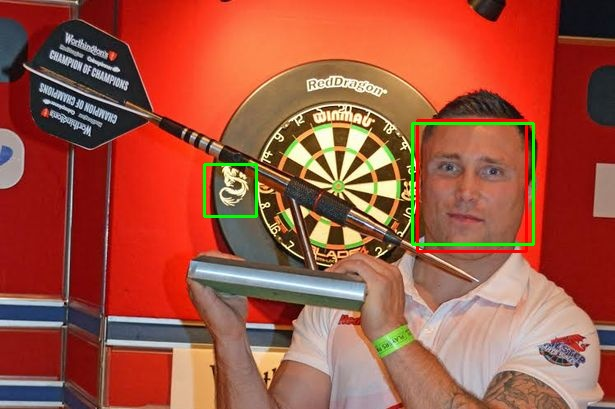
\includegraphics[width=\linewidth]{dart13-face.jpg}\par}
  \centerline{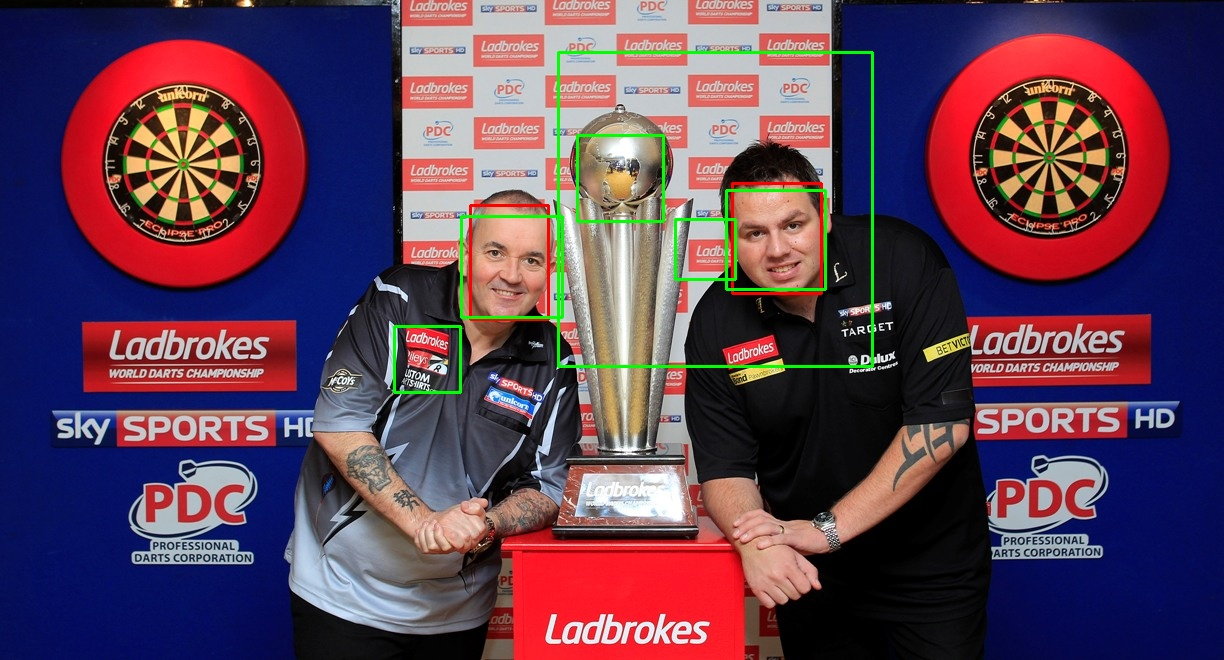
\includegraphics[width=\linewidth]{dart14-face.jpg}\par}
  \centerline{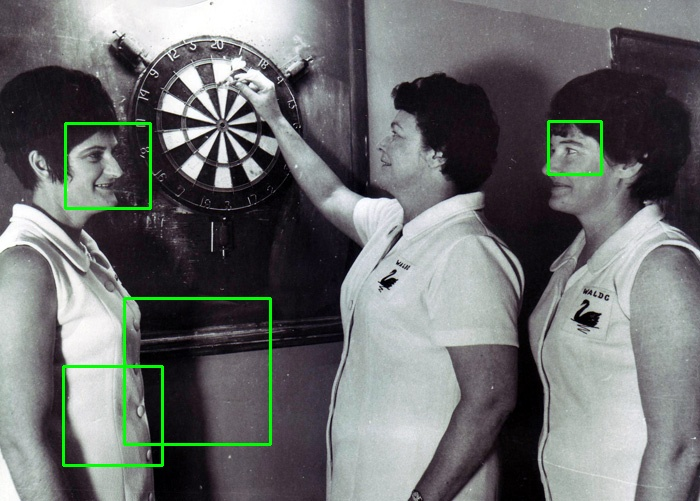
\includegraphics[width=\linewidth]{dart15-face.jpg}\par}
\end{multicols}
\captionof{figure}{Viola-Jones face detection (green) with ground truth (red)}
\label{fig:vjfaceimages}

\begin{center}
\begin{tabular}{ |p{2cm}||p{2cm}|p{2cm}| }
 \hline
 \multicolumn{3}{|c|}{Frontal face detection results} \\
 \hline
 Image name & TPR & F1-SCORE \\
 \hline
 dart4  & 1   & 1         \\
 dart5  & 1   & 0.88      \\
 dart13 & 1   & 0.666667  \\ 
 dart14 & 1   & 0.5       \\ 
 dart15 & 1   & 0         \\ 
 \hline
\end{tabular}
\captionof{table}{Viola-Jones face detection results}
\label{tab:vjfacesresults}
\end{center}

\bigskip

The results in Table \ref{tab:vjfacesresults} show the true positivity rate, TPR, and the F1 score of the Viola-Jones face detector on the input images shown in \ref{fig:vjfaceimages}. TPR is the fraction of true faces which have been detected and F1 score is given by

\[ 2 \times \frac{precision \times recall}{precision + recall} \]

where precision is the number of true positives divided by the total number of detected objects and recall is the number of true positives divided by the true number of objects in the image.

The true values used to calculate the above are determined manually for each
input image. This can results in some ambiguity as a face does not have a
strictly defined bounding region which can result in different "true" values. 

The effect of this variation in true faces is mitigated by the use of intersection over union, IOU, to determine if a true value has successfully been detected. As provided by \cite{iou} the IOU is calculated by determining 

\[ \frac{\mbox{Area of Overlap}}{\mbox{Area of Union}}\] 

for a true value and a given region classified by the detector. In this paper
for each true value we use the maximum IOU between that true value and all of
the detected values. A threshold is then definied and if the IOU is greater
than the required threadhold the true value has been detected. This threshold
is what allows for slight variations in the true values.

Similarly the Viola-Jones detector was designed as a
frontal face detector meaning a side on face would not be considered a true
value. The example in Figure \ref{fig:vjfaceimages} shows that the definition
of a side on face can also be ambiguous and therefore for in this paper the
definition requires both eyes to be fully visible. The consequence of TPR's
ambiguity is evident in the previous figure as the detector did classify one of
the side on faces and therefore its F1 would have been was reduced as result of
this not being considered a true value.

All the results in Table \ref{tab:vjfacesresults} have a TPR value of 1. This
means every valid face in the input images were detected. The Viola-Jones
method however can often have a very hight TPR. This is as a result of
"cascade" \cite{vj}implementation. When a region of the image is evaulated it
is repeatedly passed through classifiers in an overall cascade until a
classifier rejects the region of it passes thorugh all the classifiers and is
therefore on the the detected regions. Each classifier has "very high detection
rates" \cite{vj}. This means if a classifier does not have many stages then the
overall cascade will also have a very high TPR rate by not rejecting many
regions. However this will come at the cost of many false positives. In order
for a classifier to have a hight F1 score it will need a balance between high
TPR (recall) but also need a high precision and thus a low number of false
positives.


\section{Dart board detection}

Having tested the Viola-Jones detector on faces a new cascade was trained. An image of a dart board was used to generate a set of postiive images along side a set of negative images. The detector was then trained on these images and it results are shown below.

\begin{multicols}{2}

  \resizebox{\columnwidth}{!}{
  
    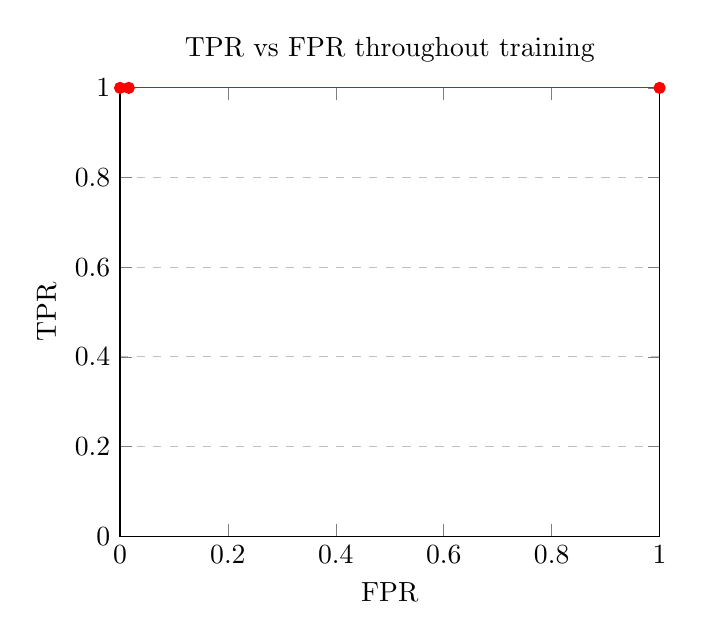
\begin{tikzpicture}
    \begin{axis}[
        title={TPR vs FPR throughout training},
        xlabel={FPR},
        ylabel={TPR},
        xmin=0, xmax=1,
        ymin=0, ymax=1,
        xtick={0, 0.2, 0.4, 0.6, 0.8, 1.0 },
        ytick={0, 0.2, 0.4, 0.6, 0.8, 1.0 },
        legend pos=north west,
        ymajorgrids=true,
        grid style=dashed,
    ]
  
    \addplot[
        color=red,
        mark=*,
        ]
        coordinates {
          (1,1)(0.0163415,1)(0.000237497,1)
        };
        
    \end{axis}
    \end{tikzpicture}
  }
 

  \resizebox{\columnwidth}{!}{
  
    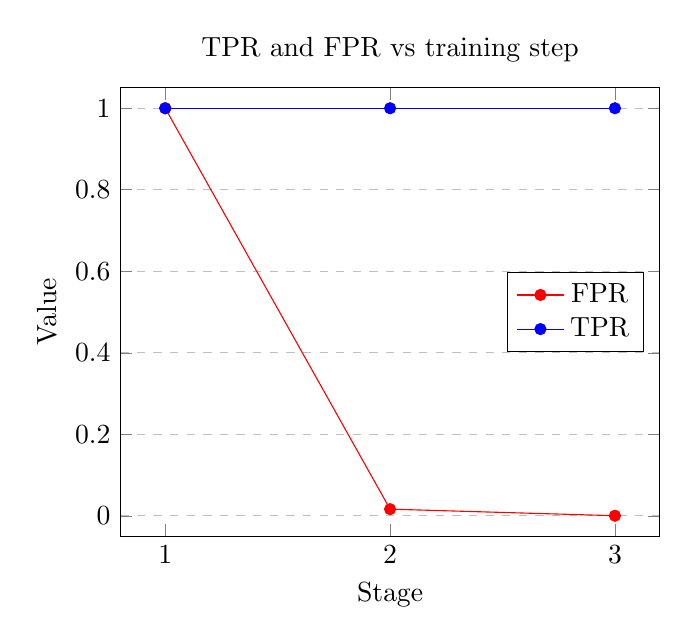
\begin{tikzpicture}
    \begin{axis}[
        title={TPR and FPR vs training step},
        xlabel={Stage},
        ylabel={Value},
        xmin=0.8, xmax=3.2,
        ymin=-0.05, ymax=1.05,
        xtick={1, 2, 3},
        ytick={0, 0.2, 0.4, 0.6, 0.8, 1.0 },
        legend style={at={(0.97,0.5)},anchor=east},
        ymajorgrids=true,
        grid style=dashed,
    ]
    
    \addplot[
        color=red,
        mark=*,
        ]
        coordinates {
          (1,1)(2, 0.0163415)(3, 0.000237497)
        };
    \addlegendentry{FPR}
    
    \addplot[
        color=blue,
        mark=*,
        ]
        coordinates {
          (1,1)(2,1)(3,1)
        };
    \addlegendentry{TPR}
        
    \end{axis}
    \end{tikzpicture}

  }
\end{multicols}
\captionof{figure}{Viola-Jones training results}
\label{fig:vjdarttraininggraph}

Figure \ref{fig:vjdarttraininggraph} shows the change in FPR and TPR throughout the
training steps. At the beginning of the training process all regions of the
image are accepted. As the training goes on more classifiers are added to the
cascade which have the oportunity to reject sections. This results in the sharp
reduction in the false positivity rates, FPR, seen in
\ref{fig:vjdarttraininggraph} as the number of negative regions which are
rejected increases. The following stage then shows another reduction in FPR for
the same reason however the reduction is far smaller as this classifier now
applies to a far smaller set of images (those which are rejected by the first
classifier are not passed on to any other classifiers) and it is performing a
more "difficult task" \cite{vj} as the previous classifiers will have filtered
out many of the neagative values.

\begin{multicols}{3}
    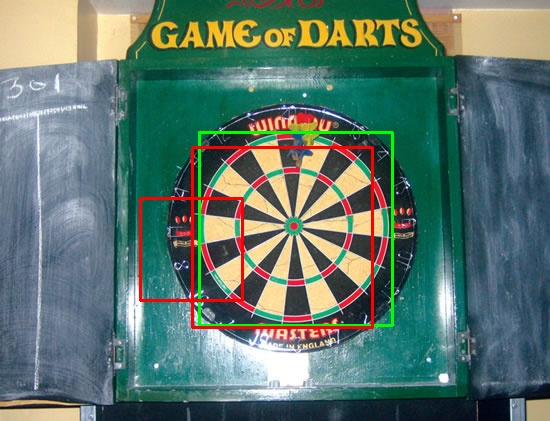
\includegraphics[width=\linewidth]{dart1-dart.jpg}\par
    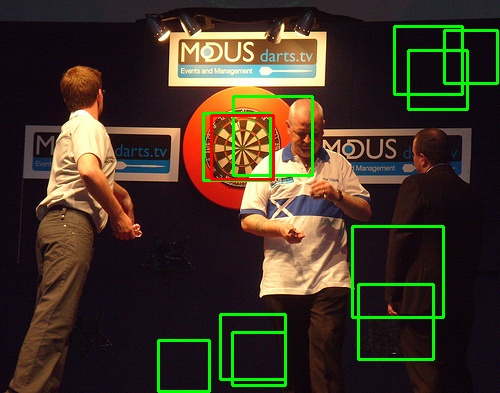
\includegraphics[width=\linewidth]{dart6-dart.jpg}\par
    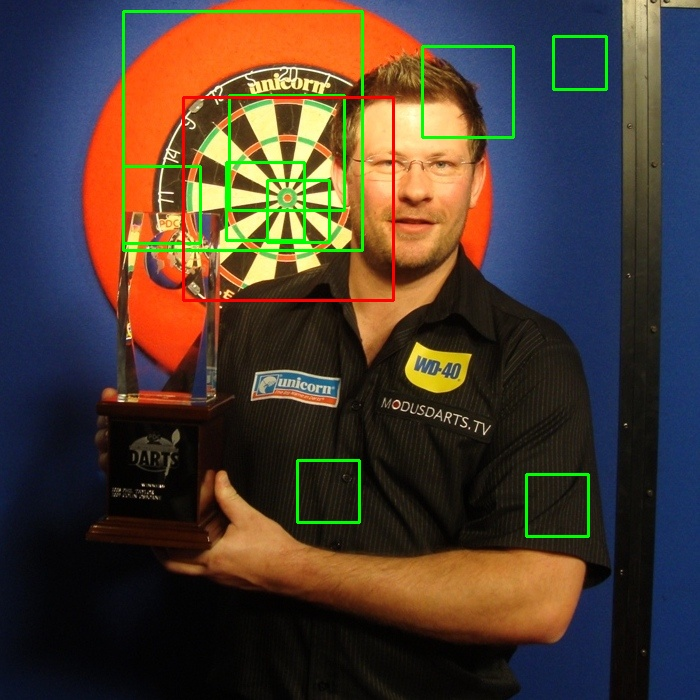
\includegraphics[width=\linewidth]{dart4-dart.jpg}\par
\end{multicols}
\captionof{figure}{Viola-Jones dartboard detection with true values}
\label{fig:vjdartsimages}


\begin{tabular}{ |p{2cm}||p{2cm}|p{2cm}| }
 \hline
 \multicolumn{3}{|c|}{Frontal face detection results} \\
 \hline
 Image name & TPR & F1-SCORE \\
 \hline
 dart1  & 1  & 0.667   \\
 dart2  & 1  & 0.25       \\
 dart3  & 1  & 0.4        \\
 dart4  & 0  & 0          \\
 dart5  & 0  & 0          \\
 dart6  & 1  & 0.182   \\
 dart7  & 0  & 0          \\
 dart8  & 0  & 0          \\
 dart9  & 0  & 0          \\
 dart10 & 0  & 0          \\
 dart11 & 0  & 0          \\
 dart12 & 0  & 0          \\
 dart13 & 0  & 0          \\
 dart14 & 0  & 0          \\
 dart15 & 1  & 0.5        \\
 \hline
 Average& 0.333333  & 0.133232    \\ 
 \hline
\end{tabular}
\captionof{table}{Viola-Jones face detection (green) with ground truth (red)}
\label{tab:vjdartstable}

The Viola-Jones algorithm described as described in \cite{vj} uses very simple feature (2, 3 or 4 rectange features). This allows the Viola-Jones algorithm to be very efficient at detecting certain objects such as faces can be difficult to scale up to more complex objects such as dartboards. This can seen in the results above. Often the classifier finds a subsection of the true dartsboards as the complex repeating pattern of the dartboard means the simple detector can not scope the full board. Similarly the results in Table \ref{tab:vjdartstable} and Figure \ref{fig:vjdartsimages}, shows that the detector has many false positives. This suggests the simple features created by the cascade are also being detected throughout the image.

The average values in Table \ref{tab:vjdartstable}, show the unreliable results of
the cascade for detecting dart boards.  It not only has a very low TPR and also
a very low F1-score suggesting there are many missed dart boards as well as
regions falsely classified. The images in Figure \ref{tab:vjdartsimages} show
the wide range of results from the classifier. a and b show successful
classifications yet b and c show the high number of false positives. It is also
noteworthy that the TPR values achieved during training were far higher than
the average achieved during testing. This is as a result of the method used to
generate positive images. These took one image of a dart board and generated
variations (via movements/rotations) on that image. This means when classifying
different types of dartboards of those with objects in the way (such as
\ref{tab:vjdartsimages} c) the classifier performs far worse.

\section{Combining Viola-Jones with hough circle detection}

From the above section it is clear that the Viola Jones detector is not well
suited to detecting dart boards and especially not to detecting the circular
shape of the dart board. In order to overcome this limitation the results from
the Viola-Jones detector can be combined with a circle hough transform. This
circle hough transform can then be used to shrink the results set and increase
the F1 score of the detector. The combination step is as follows:

\begin{itemize}
  \item Run Viola-Jones and hough circles.
  \item For every Viola-Jones results find the maximum IOU with the circles
    from hough. 
  \item If the IOU is greater than a specified threshold (0.25 in this case)
    add results from the hough to the set of final results. 
\end{itemize} 

The use of IOU with hough resulted in a large reduction in the set of results.
For the required IOU a relatively low threshold was chosen (0.4) as often the
Viola-Jones detector would find a sub section of the dart board (matching the
expected pattern) but not the circle.  For this reason the final result used
the maximum of the bounding boxes from the two detectors rather than the
Viola-Jones detector as this was more likely to encompass the full dartboard
and not just a sub section or inner circle. This removed many of the original
Viola-Jones false positives and therefore increased the F1-score dramatically.
However the limitation of this approach are clear in \ref{vjhough} which shows
the circle detector failing to detect circles with large angles to the camera
or with objects blocking sections of the circle.  This can result in a
reduction in the TPR rate of the overall detector in exchange for the reduction
in the number of false positives.

\begin{multicols}{4}
  \centerline{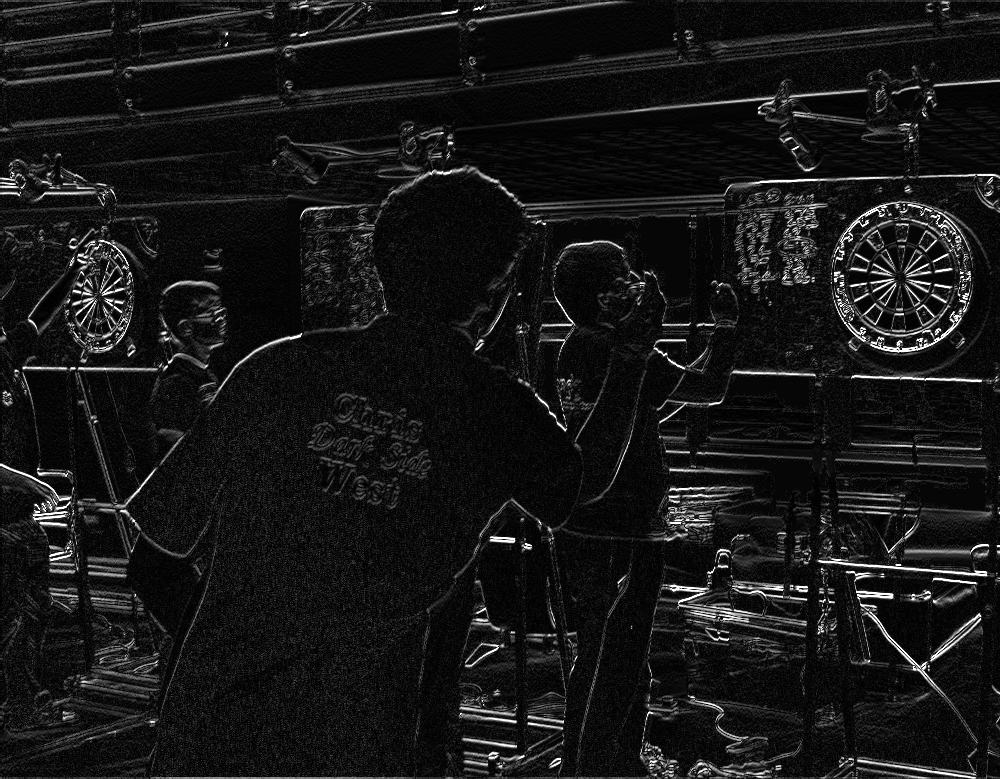
\includegraphics[width=\linewidth]{houghvj/8/gradmag.png}\par}
  \centerline{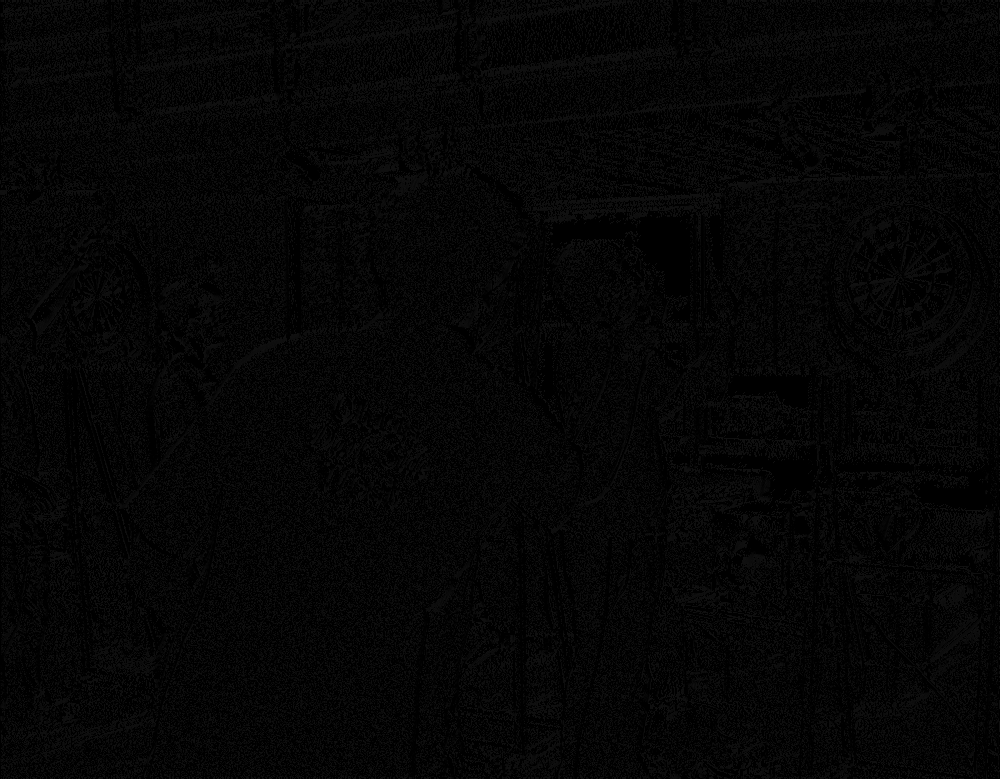
\includegraphics[width=\linewidth]{houghvj/8/graddirection.png}\par}
  \centerline{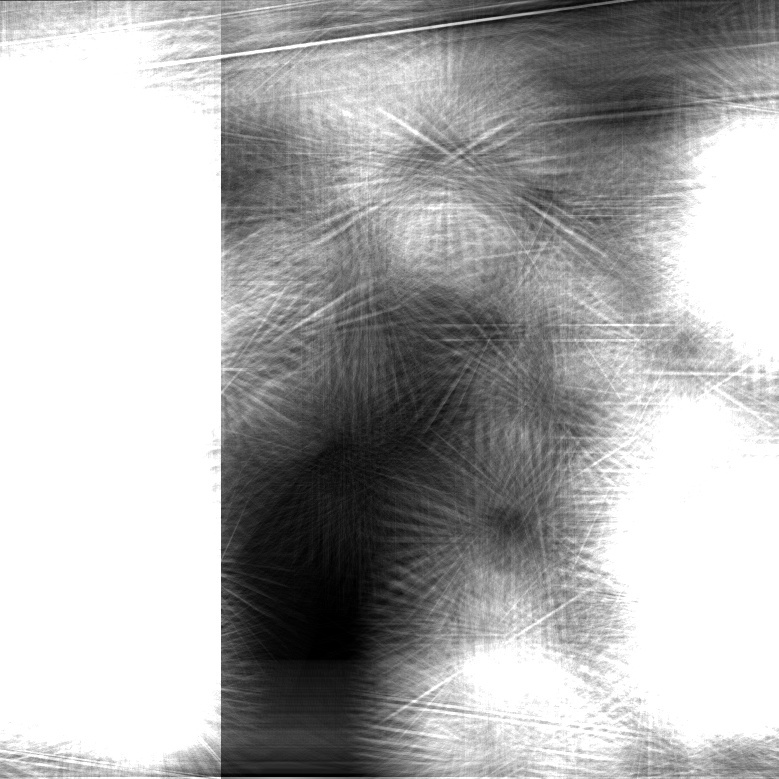
\includegraphics[width=\linewidth]{houghvj/8/cirlce-hough-space.jpg}\par}
  \centerline{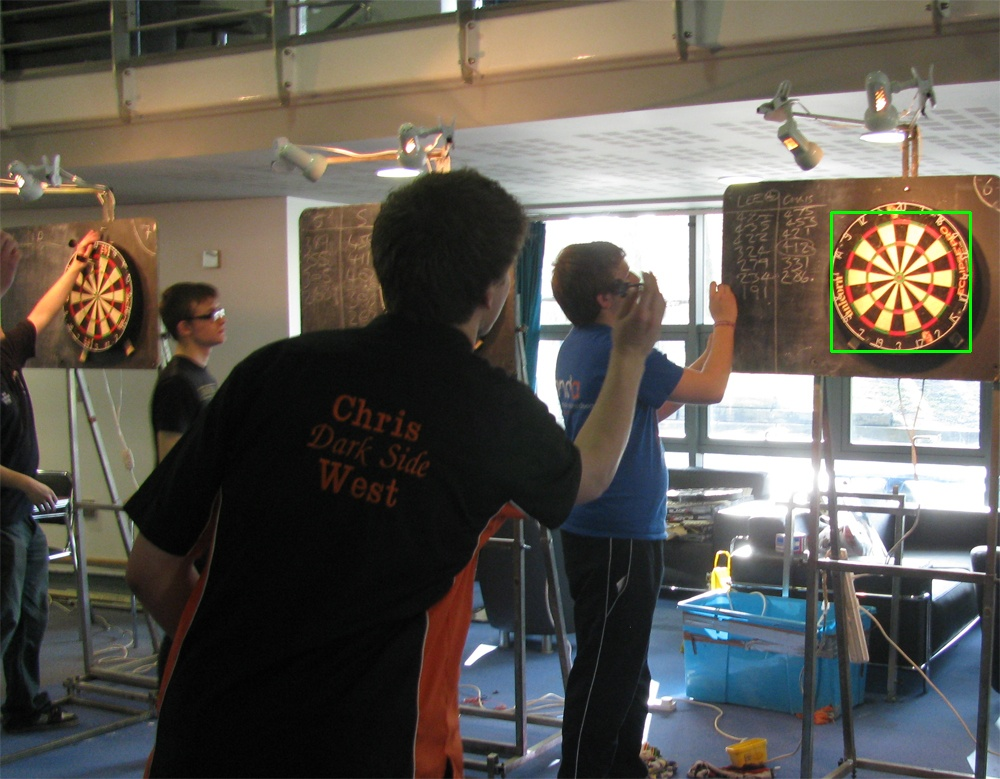
\includegraphics[width=\linewidth]{houghvj/8/final-output.jpg}\par}
\end{multicols}
\captionof{figure}{Hough circle detection on dart8.jpg}
\label{fig:hough1results}

\begin{multicols}{4}
  \centerline{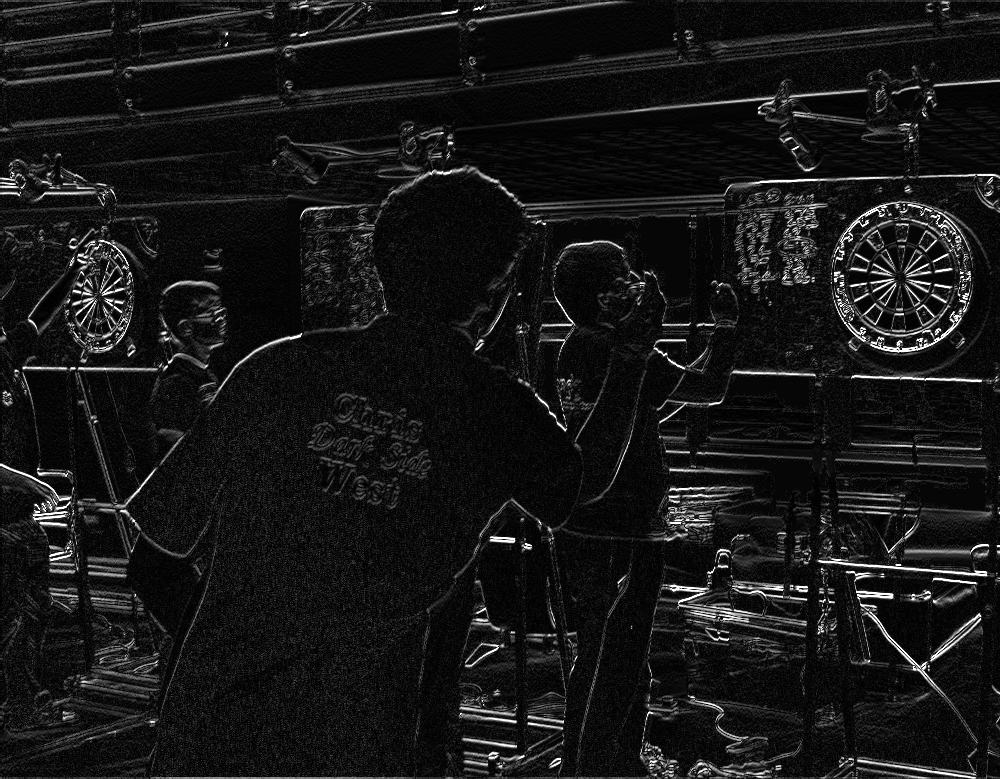
\includegraphics[width=\linewidth]{houghvj/8/gradmag.png}\par}
  \centerline{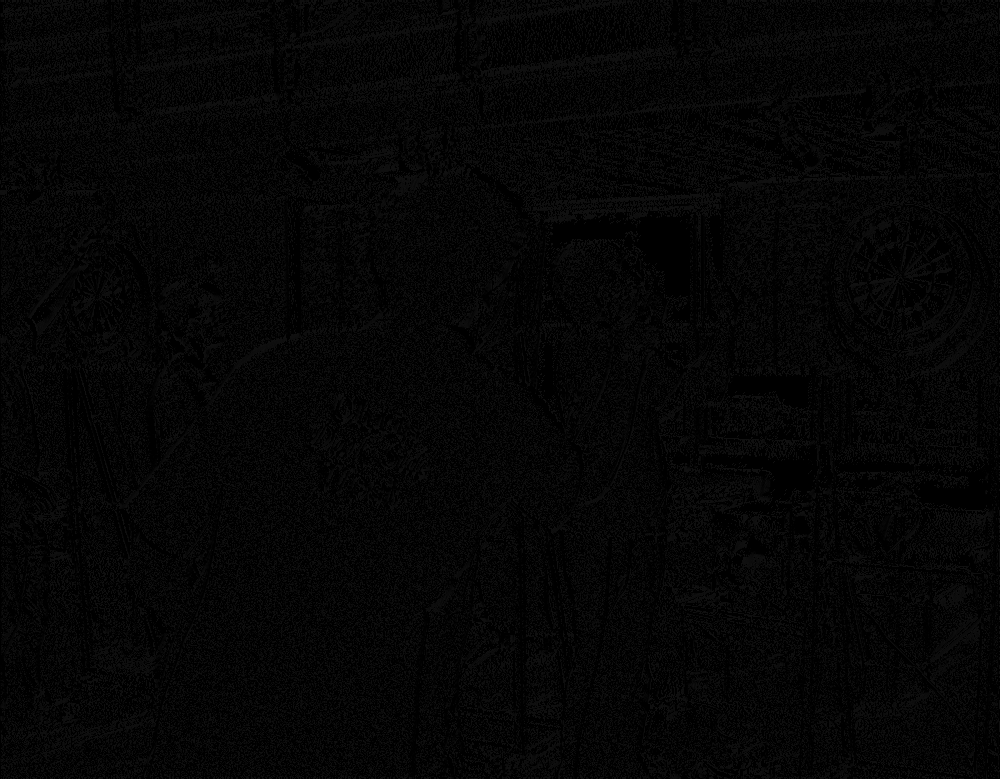
\includegraphics[width=\linewidth]{houghvj/8/graddirection.png}\par}
  \centerline{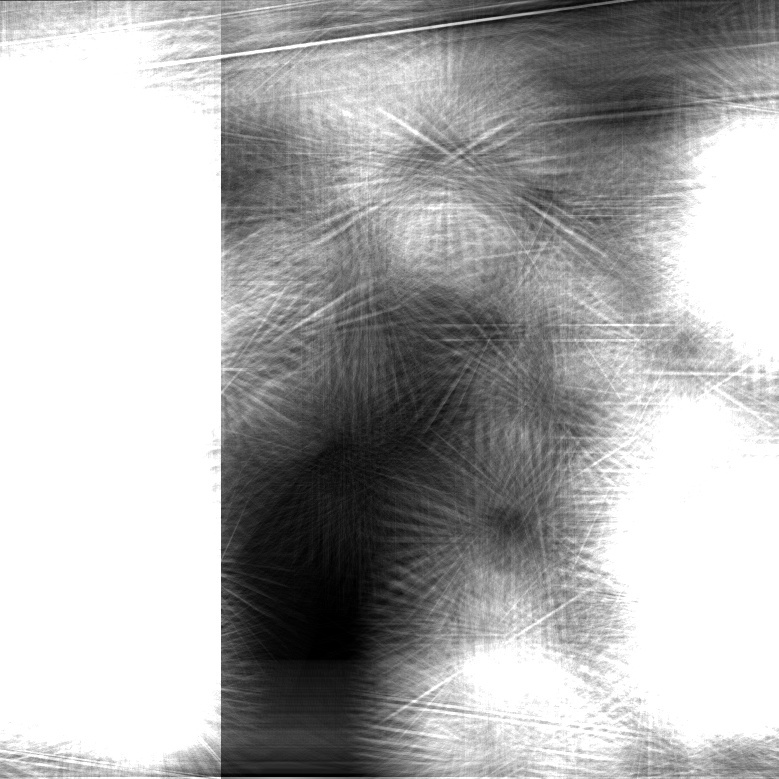
\includegraphics[width=\linewidth]{houghvj/8/cirlce-hough-space.jpg}\par}
  \centerline{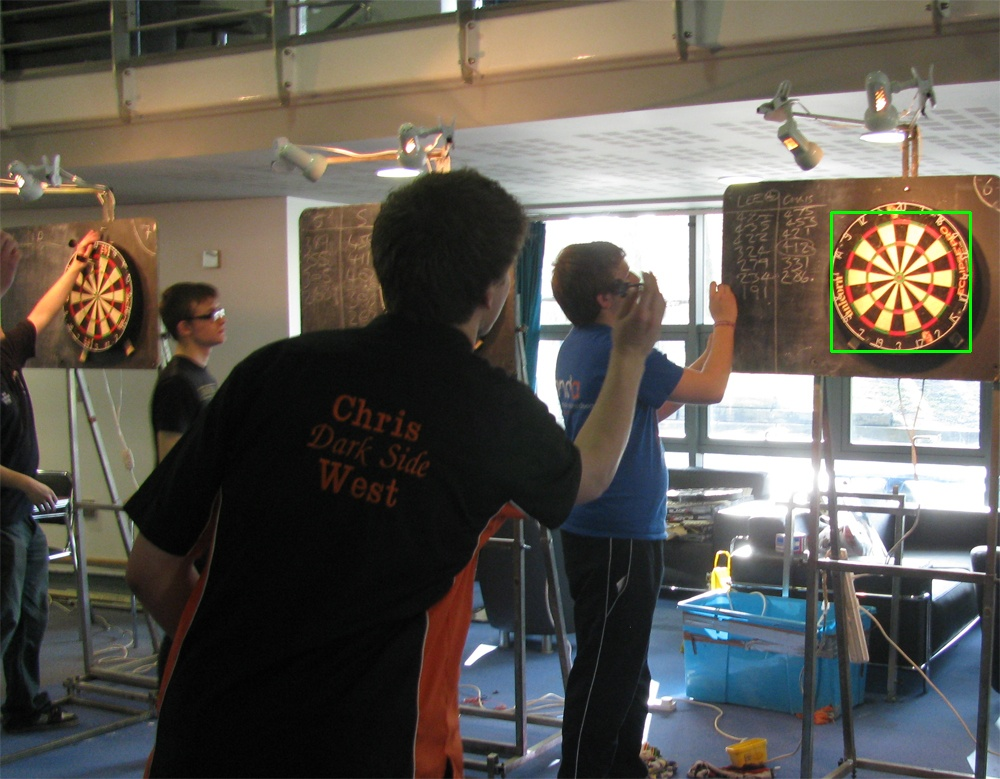
\includegraphics[width=\linewidth]{houghvj/8/final-output.jpg}\par}
\end{multicols}
\captionof{figure}{Hough circle detection on dart8.jpg}
\label{fig:hough2results}

\begin{tabular}{ |p{1.3cm}||p{1.3cm}|p{1.3cm}|p{1.3cm}|p{1.3cm}| }
 \hline
 \multicolumn{5}{|c|}{Frontal face detection results} \\
 \hline
 Image name & TPR & F1 & \(\Delta\) TPR & \(\Delta\) F1 \\
 \hline
 dart1  & 1  & 1 & 0 & + 0.333 \\
 dart2  & 1  & 0.5 & 0 & +0.25       \\
 dart3  & 1  & 0.5 & 0 & +0.1       \\
 dart4  & 0  & 0 & 0 & 0         \\
 dart5  & 1  & 1 & 0 & 0         \\
 dart6  & 0  & 0 & -1 & -0.182 \\
 dart7  & 1  & 0.5 & +1 & +0.5         \\
 dart8  & 0.5  & 0.667 & +0.5 & +0.667   \\
 dart9  & 0.5  & 0.4 & +0.5 & +0.4           \\
 dart10 & 0  & 0 & 0 & 0          \\
 dart11 & 0.333  & 0.5 & +0.333  & +0.5          \\
 dart12 & 0  & 0 & 0 & 0         \\
 dart13 & 1  & 0.4 & +1 & +0.4         \\
 dart14 & 1  & 0.5 & +1 & +0.5         \\
 dart15 & 1  & 1   & +1 & +1     \\
 \hline
 Average& 0.333333  & 0.133232 & +0.289 & 0.298   \\ 
 \hline
\end{tabular}
\captionof{table}{Viola-Jones plus hough circles detection with difference in F1 score and TPR between results in Table \ref{tab:vjdartstable}}
\label{tab:vjhoughdartstable}


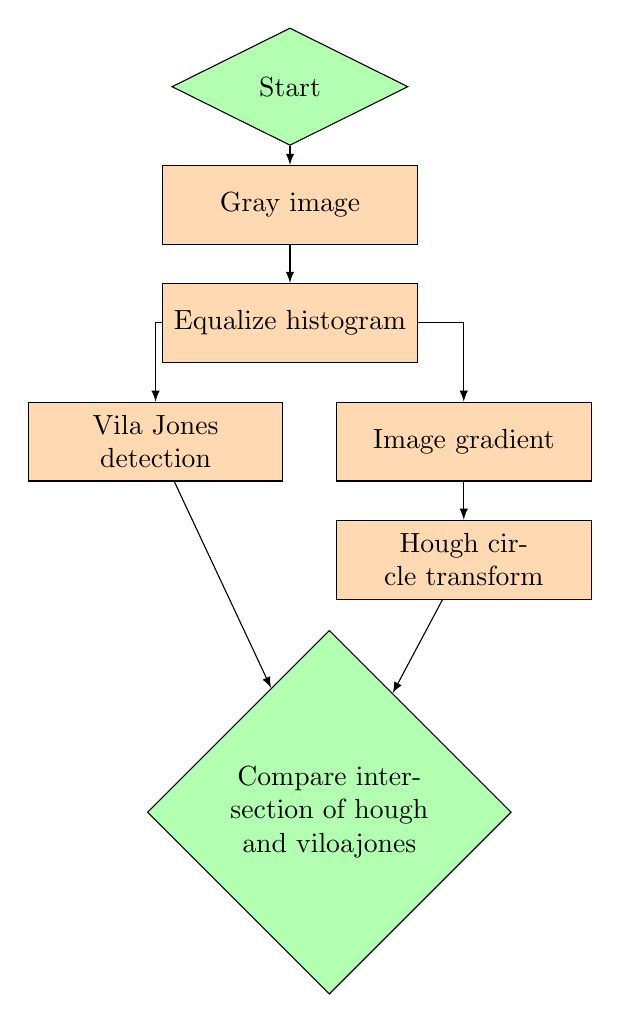
\begin{tikzpicture}[node distance=1cm]
\tikzstyle{line}=[draw]
\tikzstyle{process} = [rectangle, minimum width=3cm, minimum height=1cm, text centered, text width=3cm, draw=black, fill=orange!30]
\tikzstyle{decision} = [diamond, minimum width=3cm, text centered, text width=3cm, draw=black, fill=green!30]
\tikzstyle{sdecision} = [diamond, minimum width=3cm, draw=black, fill=green!30]
\tikzstyle{arrow}=[draw, -latex]

\node (start) [sdecision, yshift=-0.5cm] {Start};
\node (gray) [process, below of=start, yshift=-0.5cm] {Gray image};
\node (eqHist) [process, below of=gray, yshift=-0.5cm] {Equalize histogram};
\node (grad) [process, below right of=eqHist, yshift=-0.8cm, xshift=1.5cm] {Image gradient};
\node (hough) [process, below of=grad, yshift=-0.5cm] {Hough circle transform};
\node (vj) [process, below left of=eqHist, yshift=-0.8cm, xshift=-1.cm] {Vila Jones detection};
\node (threshold) [decision, below left of=hough, yshift=-2.5cm, xshift=-1.cm] {Compare intersection of hough and viloajones};

\draw [arrow] (start) -- (gray);
\draw [arrow] (gray) -- (eqHist);
\draw [arrow] (eqHist) -| (grad);
\draw [arrow] (eqHist) -| (vj);
\draw [arrow] (grad) -- (hough);

\draw [arrow] (hough) -- (threshold);
\draw [arrow] (vj) -- (threshold);

\end{tikzpicture}



\end{multicols}{2}

\bibliographystyle{unsrt}
\bibliography{report}

\end{document}
